\documentclass[]{article}
\usepackage{lmodern}
\usepackage{amssymb,amsmath}
\usepackage{ifxetex,ifluatex}
\usepackage{fixltx2e} % provides \textsubscript
\ifnum 0\ifxetex 1\fi\ifluatex 1\fi=0 % if pdftex
  \usepackage[T1]{fontenc}
  \usepackage[utf8]{inputenc}
\else % if luatex or xelatex
  \ifxetex
    \usepackage{mathspec}
  \else
    \usepackage{fontspec}
  \fi
  \defaultfontfeatures{Ligatures=TeX,Scale=MatchLowercase}
\fi
% use upquote if available, for straight quotes in verbatim environments
\IfFileExists{upquote.sty}{\usepackage{upquote}}{}
% use microtype if available
\IfFileExists{microtype.sty}{%
\usepackage{microtype}
\UseMicrotypeSet[protrusion]{basicmath} % disable protrusion for tt fonts
}{}
\usepackage[unicode=true]{hyperref}
\hypersetup{
            pdfborder={0 0 0},
            breaklinks=true}
\urlstyle{same}  % don't use monospace font for urls
\usepackage{graphicx,grffile}
\makeatletter
\def\maxwidth{\ifdim\Gin@nat@width>\linewidth\linewidth\else\Gin@nat@width\fi}
\def\maxheight{\ifdim\Gin@nat@height>\textheight\textheight\else\Gin@nat@height\fi}
\makeatother
% Scale images if necessary, so that they will not overflow the page
% margins by default, and it is still possible to overwrite the defaults
% using explicit options in \includegraphics[width, height, ...]{}
\setkeys{Gin}{width=\maxwidth,height=\maxheight,keepaspectratio}
\IfFileExists{parskip.sty}{%
\usepackage{parskip}
}{% else
\setlength{\parindent}{0pt}
\setlength{\parskip}{6pt plus 2pt minus 1pt}
}
\setlength{\emergencystretch}{3em}  % prevent overfull lines
\providecommand{\tightlist}{%
  \setlength{\itemsep}{0pt}\setlength{\parskip}{0pt}}
\setcounter{secnumdepth}{0}
% Redefines (sub)paragraphs to behave more like sections
\ifx\paragraph\undefined\else
\let\oldparagraph\paragraph
\renewcommand{\paragraph}[1]{\oldparagraph{#1}\mbox{}}
\fi
\ifx\subparagraph\undefined\else
\let\oldsubparagraph\subparagraph
\renewcommand{\subparagraph}[1]{\oldsubparagraph{#1}\mbox{}}
\fi

% set default figure placement to htbp
\makeatletter
\def\fps@figure{htbp}
\makeatother


\date{}

\begin{document}

Morbo di Dupuytren

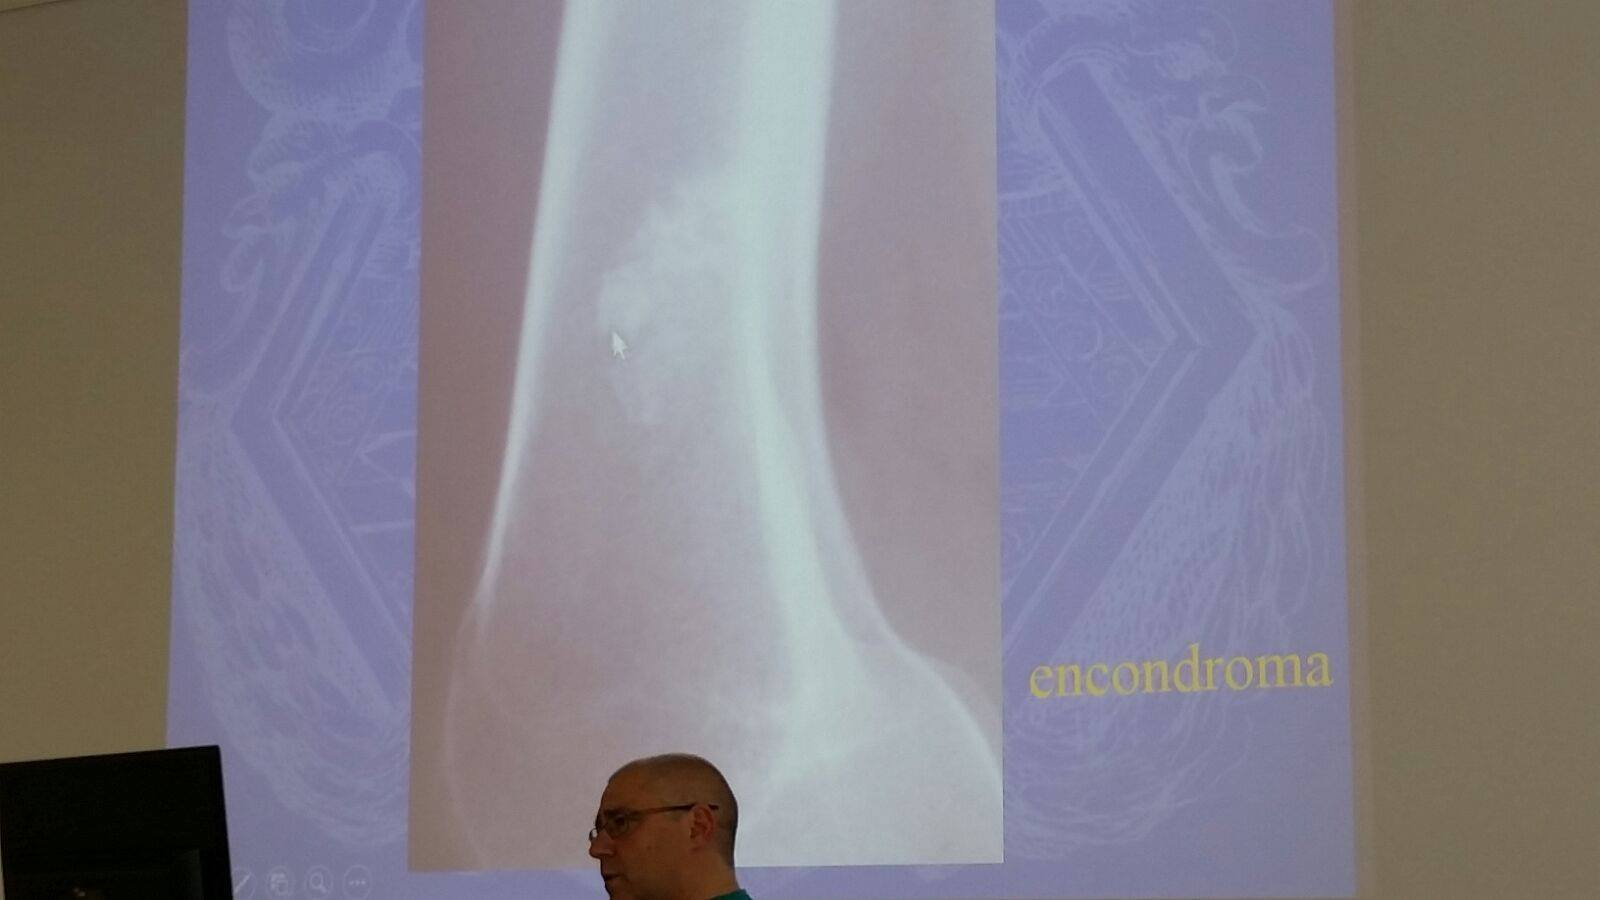
\includegraphics[width=4.02292in,height=2.24028in]{media/image1.jpeg}Il
morbo di Dupuytren è una patologia più frequente negli \textbf{uomini}
che non nelle donne, la cui eziopatogenesi non è ancora conosciuta in
maniera approfondita (E' una malattia degenerativa che coinvolge
fibroblasti e miofibroblasti, dovuto ad un primitivo danno vascolare
(ischemia microvascolare), si assiste alla proliferazione dei
fibroblasti lungo linee di stress meccanico, con formazione di strutture
cordoniformi nella fascia palmare).

Può esserci una componente familiare ed alcuni hanno associato lo
sviluppo di questa patologia a lavori che comportano vibrazioni a
livello della mano (es utilizzo di martelli pneumatici), o da patologie
come diabete, alcolismo, o farmaci tipo "Gardenale" ecompare di solito
dopo i 40 anni.

È caratterizzata da un \emph{progressivo ispessimento e da una
progressiva retrazione delle bandelette dell'aponeurosi palmare} che
possono far retrarre e far flettere le dita sia in corrispondenza
dell'articolazione metacarpofalangea che dell'articolazione
interfalangea.

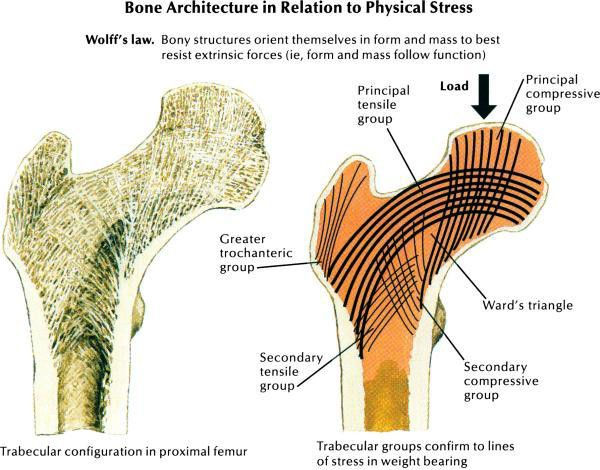
\includegraphics[width=3.03611in,height=2.02917in]{media/image2.jpeg}Generalmente
si presenta con la formazione di noduli fibrosi sottocutanei che
diventano poi cordoni sempre sottocutanei. La patologia colpisce
preferibilmente il \emph{quarto e il quinto raggio della mano} e meno
frequentemente i primi tre raggi. Spesso è bilaterale e si può
sviluppare anche alla pianta del piede. Bisogna sempre chiedere al
paziente se ha le stesse problematiche anche alla pianta del piede, come
\textbf{noduli o cordoni duri} che determinano la retrazione
dell'aponeurosi plantare. Nei maschi può essere associata a una
\emph{retrazione della tonaca albuginea del pene.} Queste complicanze
che riguardano piede e pene non sono frequenti ma devono essere tenute
in considerazione.

Diagnosi

La diagnosi è per questo tipo di patologia è essenzialmente clinica,
bisogna vedere la mano e palpare il nodulo o il cordone che si sente
molto bene in corrispondenza del palmo. La velocità di progressione da
nodulo a cordone e da dito esteso a dito flesso e a dito flesso
totalmente non è assolutamente prevedibile, può essere velocissima
oppure il paziente può restare stabile per anni senza avere nessun tipo
di retrazione. Molto spesso in ambulatorio arrivano degli stadi iniziali
di morbo di Dupuytren che noi non trattiamo chirurgicamente.

Trattamento

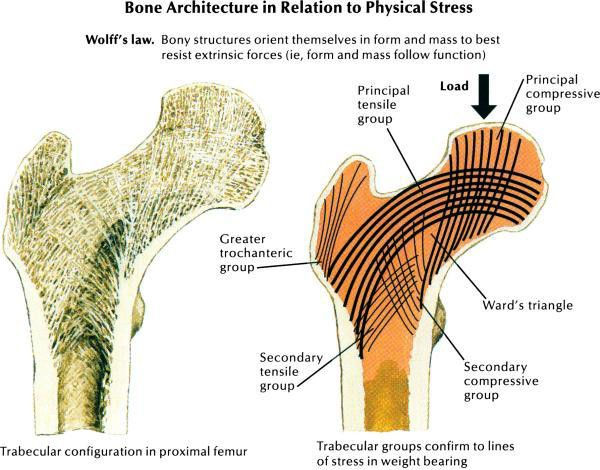
\includegraphics[width=2.60208in,height=3.40764in]{media/image3.jpeg} Il
trattamento iniziale infatti è di tipo astensionistico ed osservazionale
a domicilio; si dice al paziente di guardare se il nodulo diventa
cordone, se inizia a retrarsi e a piegarsi il dito, e in quel caso si va
verso un ipotesi chirurgica.

La chirurgia è nella maggior parte dei casi a cielo aperto e
l'intervento viene fatto possibilmente con occhiali da microchirurgia.
Si fanno delle incisioni curvilinee a zig zag al di sopra dei cordoni o
dei noduli, e si va a togliere l'aponeurosi retratta ossia quella
patologica \emph{( N.B. l'immagine a lato con i nomi delle incisioni è a
solo scopo illustrativo}).

L'intervento si chiama perciò di \textbf{aponeurectomia selettiva}
quindi:

\begin{itemize}
\item
  Anestesia generale o loco-regionale del braccio
\item
  Ricovero ospedaliero per 24\textasciitilde{}48ore;
\item
  Larga apertura,unica o multipla,delle dita e del palmo della mano per
  l'asportazione della
\end{itemize}

fascia palmare ispessita e retratta;

\begin{itemize}
\item
  Cicatrizzazione cutanea di 2settimane;
\item
  Riabilitazione di 1\textasciitilde{}2mesi;
\item
  Utilizzo di tutore notturno per le dita operate;
\item
  Sospensione del lavoro di 1\textasciitilde{}2mesi per i lavoratori
  manuali
\end{itemize}

In alcuni casi molto selezionati si potrebbe fare una
\textbf{aponeurectomia percutanea}, ossia con un ago viene tagliato il
cordone fibroso per recuperare l'estensione del dito è una tecnica
mini-invasiva, consiste nella sezione multipla della sclerosi
aponeurotica, ispessita e retratta, eseguita con un ago , abbiamo:

\begin{itemize}
\item
  Anestesia locale
\item
  Senza ricovero,in day-hospital;
\item
  Tecnica mini-invasiva,senza apertura delle dita e del palmo della
  mano: l'ago taglia in sotto-
\item
  cutaneo la fascia palmare retratta in diversi punti e quindi si
  allunga normalmente;
\item
  Nessun tempo di cicatrizzazione;
\item
  Minima riabilitazione;
\item
  Nessuna sospensione del lavoro;
\item
  Raramente si utilizzerà un tutore notturno.
\end{itemize}

Questa tecnica è, purtroppo, molto spesso dimenticata o non conosciuta
dagli specialisti, per cui troppi malati non possono beneficiarne.

Possono essere utilizzati anche dei \textbf{farmaci} (non in commercio
in Italia) che vengono iniettati nel sottocute e ``sciolgono'' il
cordone aponeurotico. Nella maggior parte dei casi però si interviene
chirurgicamente con l'aponeurectomia selettiva. I cordoni fibrosi
tendono ad inglobare i nervi digitali che danno la sensibilità alle
dita, quindi l'intervento di aponeurectomia si fa primariamente sui
nervi e poi sulle altre strutture, ossia devono essere prima isolati,
scollati e protetti i fasci vascolonervosi della mano, e poi viene tolto
il fascio stesso.

Come complicanza ci può essere una lesione vascolonervosa, ad esempio
del nervo digitale, perché scollando può essere tagliato o lesionato.
Altre complicanze presenti dopo questo intervento sono le recidive che
si suddividono in:

\begin{itemize}
\item
  \emph{recidive vere}, dovute al fatto che non viene tolta tutta
  l'aponeurosi patologica e di conseguenza si riforma un cordone che
  retrae. In questo caso bisogna riaprire e togliere l'aponeurosi
  patologica.
\item
  \emph{recidive false}, dovute ad una retrazione successiva
  all'intervento chirurgico e legata alla formazione di una cicatrice
  aberrante o di un \textbf{cheloide} che determina la retrazione del
  raggio e del dito che è stato operato. In questo caso, grazie alla
  chirurgia plastica, si possono fare interventi di allungamenti e
  plastiche a zeta per ritornare ad avere il dito esteso.
\end{itemize}

A volte arrivano in ambulatorio pazienti in uno stadio avanzato, ad
esempio anziani che riferiscono di aver sempre avuto un dito flesso e
che non ha dato alcun fastidio, ma solo qualche limitazione nei
movimenti quotidiani (es afferrare oggetti, mettere i guanti). In questo
caso c'è l'indicazione chirurgica, stiamo parlando però di persone che
hanno questa rigidità in flessione da anni, di conseguenza tutte le
strutture vascolo nervose si sono retratte e accorciate. Può capitare
che ridando la lunghezza e l'estensione giusta del raggio possano venire
stirati e rotti i nervi e ci possono quindi essere delle crisi
vascolari. In questi casi si può dire al paziente che si può fare un
tentativo per recuperare l'estensione, se vanno in crisi vascolare può
darsi che si debba amputare il dito. In alcuni casi estremi si
preferisce amputare subito piuttosto che fare il raddrizzamento e poi
eventualmente l'amputazione. Questo non è un intervento da anestesia
locale, ma viene fatto con un \textbf{anestesia plessica}. Di solito il
paziente resta ricoverato una notte e a seconda della gravità del morbo
di Dupuytren e di conseguenza del grado di retrazione in flessione delle
dita, il decorso post operatorio è più o meno facile.

Nel decorso post-operatorio di una forma iniziale:

\begin{itemize}
\item
  si fa un bendaggio,
\item
  si cura la cicatrice,
\item
  dopo 15 giorni si tolgono i punti,
\item
  infine si fa un trattamento della cicatrice che consiste in un
  massaggio desensibilizzante per far riassorbire l'ematoma,
\item
  recupero progressivo della mobilità.
\end{itemize}

Nei casi più gravi (quando c'è una flessione abbastanza importante prima
dell'intervento chirurgico):

\begin{itemize}
\item
  si associa il posizionamento di una stecca gessata in estensione per
  mantenere le dita dritte per i primi 15 giorni da tenere tutto il
  giorno,
\item
  alla rimozione dei punti può iniziare la fisioterapia per il recupero
  dell'articolarità e il trattamento fisioterapico della ferita,
\item
  si possono fare dei tutori su misura amovibili dorsali, ossia dalla
  parte opposta della ferita in estensione, che inizialmente vengono
  mantenuti negli intervalli tra le sedute fisioterapiche,
\item
  dopo 1 mese dall'intervento il tutore deve essere tenuto di notte per
  almeno 6-8 mesi dall'intervento.
\end{itemize}

Sindrome di De Quervain

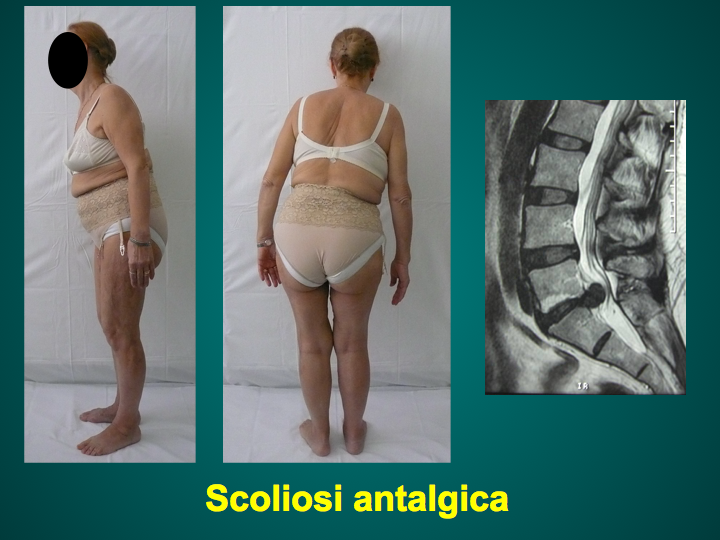
\includegraphics[width=2.44097in,height=1.74722in]{media/image4.png}Altra
patologia della mano abbastanza frequente è la sindrome di De Quervain
che per definizione è una \textbf{tenosinovite o tenovaginalite
stenosante} dei tendini:

\textbf{1}-\textbf{estensore breve }

\textbf{2-abduttore lungo del pollice}

tendini che attraversano il primo compartimento osteo-fibroso degli
\textbf{estensori}, presente sulla superficie dorsale del radio.

I tendini estensori decorrono a livello del radio distale in canali
osteo-fibrosi, che vanno a costituire i sei compartimenti degli
estensori

\begin{enumerate}
\def\labelenumi{\arabic{enumi}.}
\item
  Il primo compartimento è quello che interessa il morbo di De Quervain
  e al suo interno passano l‟estensore breve del pollice e l‟abduttore
  lungo del pollice;
\item
  Il secondo compartimento accoglie gli estensori radiali (breve e
  lungo) del carpo ;
\item
  Il terzo compartimento è quello dell‟estensore lungo del pollice;
\item
  Il quarto compartimento contiene l‟estensore comune delle dita e
  l‟estensore proprio dell‟indice;
\item
  Il quinto compartimento contiene l‟estensore proprio del V dito;
\item
  Nel sesto e ultimo compartimento passa l‟estensore ulnare del carpo.
\end{enumerate}

I tendini estensori passano attraverso queste strutture e sono ricoperti
dalle loro guaine sinoviali: quando si ha una compressione dei tendini
compresi nel primo compartimento si parla di morbo di De Quervain.

Se si abduce il primo dito si vede un tendine, questo è
\emph{l'estensore lungo del pollice}, se vi avvicinate verso il palmo
della mano a livello dell'articolazione del polso si sentono altri due
tendini o un cordone composto da quei tendini; questo è quello che
riguarda il morbo di De Quervain, ovvero l'estensore breve e l'abduttore
lungo. Tutti gli estensori a livello del dorso del polso sono contenuti
all'interno di canali osteofibrosi; la loro presenza permette che i
tendini scorrano al loro interno durante l'estensione del polso e non si
stacchino dall'osso. Non c'è quindi l'effetto corda d'arco. Quando i
tendini, per vari motivi (ad es per la degenerazione di una corda
tendinea o per un processo infiammatorio delle guaine peritendinee),
fanno fatica a scorrere all'interno di questi canali osteofibrosi, si
possono avere delle tendinovaginaliti stenosanti ed è il caso del morbo
di De Quervain. Questa patologia è più frequente nelle \textbf{donne}
,(Rapporto M:F 1:6) che non negli uomini, ed è correlata a quelle
\textbf{attività lavorative o ludiche} che comportano un estensione
continua del pollice, in particolare è caratteristica delle donne che
lavorano molto con le dita, che abbiano attività caratterizzate da
movimenti ripetitivi di abduzione radiale del pollice, con simultanea
inclinazione ulnare del polso. La fascia d'età più colpita coincide con
la quarta e quinta decade.

Clinica

Dal punto di vista clinico è presente un dolore elettivo a livello della
stiloide radiale,punto in cui decorrono i tendini sopracitati,
esacerbato dalla digitopressione e dalla estensione contro resistenza.
Ci può essere una tumefazione, e a volte può essere presente anche un
crepitio, legato al fatto che il tendine con la sua guaina rigonfia fa
fatica a scorrere e in questo canale si può saltuariarmente sentire un
\emph{crik-crok , se nel movimento di flesso-estensione del pollice, si
appoggiano le dita lungo il decorso del tendine, si possono sentire dei
piccoli ``sfrusciamenti'', causati della guaina del tendine che scorre.
La diagnosi è clinica e c‟è un test specifico: }

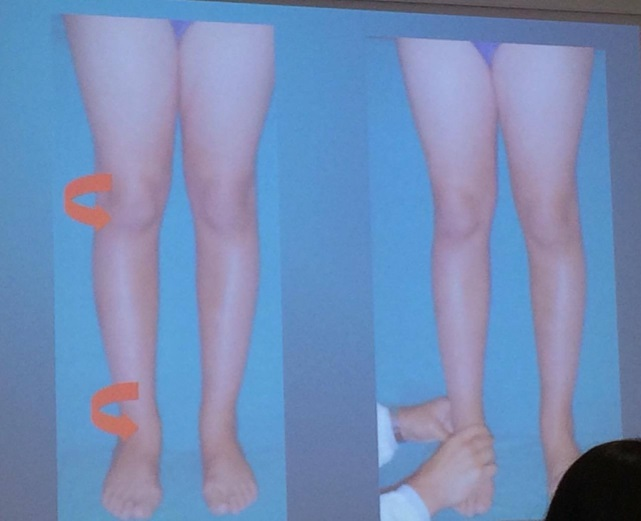
\includegraphics[width=4.22917in,height=2.02708in]{media/image5.jpeg}

Il \textbf{Test di Finkelstein} è un test specifico in cui si chiede al
paziente di mettere il pollice in questa posizione, di chiudere le altre
dita al di sopra del pollice e di inclinare ulnarmente il polso.
\emph{Questa inclinazione ulnare attiva o passiva fatta da un
esaminatore determina un dolore caratteristico a livello della stiloide
radiale} che si può irradiare lungo il decorso dei due tendini e dei due
ventri muscolari.

Diagnosi

La diagnosi è primariamente clinica, di solito per confermarla si
possono fare degli esami strumentali e in particolare uno studio
\textbf{ecografico} bilaterale dei polsi è sufficiente per mettere in
evidenza questa patologia,può mettere in evidenza un‟infiammazione dei
tendini interessati.

A volte è giusto fare anche una \textbf{radiografia} associata perchè
possono esserci delle protuberanze o delle esostosi della stiloide
radiale che possono favorire l'insorgenza di questa patologia,a volte ci
possono essere degli osteofiti della stiloide radiale che vanno a
comprimere i tendini, in tal caso il trattamento sarà chirurgico.

Trattamento

Il trattamento come sempre è di tipo conservativo; si possono usare dei

\begin{itemize}
\item
  \textbf{Tutori su misura} che mette a riposo l'articolazione e il dito
\end{itemize}

dell'articolazione del polso e del primo raggio.

\begin{itemize}
\item
  Il passaggio successivo, che ha un risultato positivo in una buona
  percentuale di pazienti (50-80\%), è quello di fare delle
  \textbf{infiltrazioni con corticosteroidi locali}, bisogna essere però
  in grado di andare con l'ago tra il tendine e il canale osteofibroso
  ed iniettare il cortisonico non dentro al tendine ma attorno ad esso(
  i corticosteroidi dovranno essere iniettati in zona peritendinea e non
  intratendinea, arrivando al di sotto della guaina che copre il
  tendine).
\end{itemize}

Procedura:

1-palpo il tendine;

\begin{quote}
2-inserisco l‟ago che arriva in profondità, deve superare la guaina
tendinea;

3- passivamente muovo il dito, se l‟ago ``sbandiera'' vuol dire che ho
punto il tendine, se invece rimane perpendicolare vuol dire il tendine
non è stato punto e posso iniettare.

4 L‟infiltrazione deve essere peritendinea, quindi devo superare la
guaina tendinea, ma non andare

dentro il tendine!
\end{quote}

\begin{enumerate}
\def\labelenumi{\arabic{enumi}.}
\item
  3-Qualora il trattamento conservativo non abbia successo si può fare
  un \textbf{trattamento chirurgico} che consiste nella
  \emph{liberazione del tendine dalla compressione} presente all'interno
  del canale osteofibroso interessato. Si fa quindi un intervento di
  \textbf{tenolisi}, di liberazione del tendine, che è svolto in
  anestesia locale e non prevede un ricovero, dopo qualche ora il
  paziente può tornare a casa. Di solito si preferisce fare non tanto un
  incisione longitudinale lungo il decorso dei tendini dei muscoli, ma
  piuttosto un \emph{incisione trasversale} centrata sulle pliche
  dorsali del radio in quanto darà una cicatrice molto più bella.
  Bisogna stare attenti nel fare il taglio trasversale in quanto c'è un
  ramo sensitivo del nervo radiale che passa a questo livello e che dà
  la sensibilità dorsale in tutta questa zona. Se tagliato o lesionato
  può dare ipoanestesia della zona interessata ma può anche causare dei
  neuromi dolorosi da amputazione del nervo. Questa patologia può essere
  mono o bilaterale, essendo però legata a prese di forza o movimenti
  ripetuti di solito interessa la mano dominante.
\end{enumerate}

Dito a scatto

Esiste un'altra patologia molto frequente che è nominata dito a scatto;
si tratta di una una \textbf{\emph{tenovaginite stenosante che interessa
i flessori delle dita}}. Lo scatto può essere causato da un
restringimento del canale oppure dal fatto che il tendine infiammato
faccia fatica a scorrere in corrispondenza della base del dito. Questa
stenosi si verifica in corrispondenza della \textbf{superficie volare
del palmo della mano a livello della testa dei metacarpi}, dove è
presente una struttura che è la prima puleggia circolare chiamata anche
\textbf{puleggia A1}.

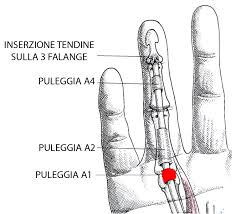
\includegraphics[width=3.24236in,height=3.77361in]{media/image6.png}

Il flessore superficiale si inserisce volarmente alla base della seconda
falange, il flessore profondo si inserisce volarmente alla base della
terza falange; la loro azione combinata determina la possibilità di fare
il pugno. I tendini flessori scorrono all'interno di canali fibrosi e
per compiere l'azione flessoria e scorrere adesi all'osso sono ricoperti
dal strutture fibrose che si chiamano pulegge. Se non avessimo le
pulegge avremmo un effetto a corda d'arco durante il movimento, e quindi
i tendini si staccherebbero dall'osso al di sotto della cute. A volte il
tendine fa fatica a scorrere a livello della puleggia A1, questa
difficoltà determina una sensazione di scatto (clik-clok) quando il
paziente cerca di flettere il dito. Lo scatto può essere riducibile,
ovvero dopo la flessione si riesce a raddrizzare, ma può anche diventare
irriducibile. In casi estremi il paziente arriva con il dito flesso e
per ridurlo deve aiutarsi con l'altra mano perchè non riesce a
raddrizzarlo da solo, e di solito questo è un gesto doloroso.

Eziologia

Possono esserci:

\begin{itemize}
\item
  \textbf{forme congenite}, nei neonati fino a uno o due anni colpiscono
  il pollice e si parla di pollice a scatto congenito e può essere
  bilaterale.
\end{itemize}

Il bimbo si presenta in ambulatorio con la falange distale del pollice
atteggiata in flessione, dura, non si riesce a raddrizzare. Avrà
caratteristicamente a livello della base della falange un nodulo di
solito duro.

\begin{itemize}
\item
  \textbf{forme non congenite},sono le forme più frequenti ,colpiscono
  gli adulti e interessano il primo, il terzo e il quarto dito. Il dito
  può muoversi e sentire lo scatto ma si può anche bloccare dando uno
  scatto doloroso. Ci possono essere dei quadri progressivamente più
  gravi.
\end{itemize}

L'incidenza di questa patologia presenta un picco tra i 50 e i 60 anni,
ed è molto maggiore, fino a sei volte nel sesso femminile. Le dita più
colpite sono in ordine decrescente: pollice, anulare, medio, mignolo e
indice.

Diagnosi

Anche in questo caso la diagnosi è prevalentemente clinica, ossia il
paziente ha male alla palpazione del palmo della mano in corrispondenza
della testa del metacarpo, e alla flessione attiva e passiva si sente
uno scatto. Molto spesso c'è un rigonfiamento, una specie di nodulo, in
corrispondenza della puleggia interessata, nelle forme conclamate, il
dito rimane flesso, bloccato in flessione e il paziente per estendere il
dito dovrà applicare una forza importante .

L'esecuzione di ecografie e radiografie sono inutili.

Il fenomeno dello scatto è dovuto all'incongruenza tra le dimensioni dei
tendini flessori e della guaina fibrosa a livello della puleggia A1. Si
ritiene che durante le prese di forza, l'attrito contro la puleggia
favorisca uno scompaginamento delle fibre dei tendini, analogo a quanto
può accadere, quando un filo viene tirato attraverso la cruna di un ago.
Ciò determina la formazione di un nodulo reattivo nel conteso del
tendine.

Wolfe ha proposto una \textbf{\emph{classificazione}} del dito a scatto
in base all'evoluzione clinica secondo lo schema seguente:

\begin{quote}
 ~Grado I: il paziente riferisce dolore e scatto, l'esame obiettivo non
evidenzia lo scatto ma solo dolorabilità elettiva a livello della
puleggia A1;
\end{quote}

\begin{itemize}
\item
  ~Grado II: presenza di scatto, l'estensione attiva è possibile;
\item
  ~Grado III: presenza di scatto con possibilità d'estensione solo
  passiva (III A) o impossibilità di
\end{itemize}

\begin{quote}
flessione attiva (III B);

 ~Grado IV: retrazione irriducibile in flessione.
\end{quote}

Trattamento

Nella maggior parte dei casi il trattamento che porta ad una risoluzione
del problema è \textbf{l'iniezione con corticosteroidi}, che viene
effettuato attorno alla puleggia e sotto alla puleggia. Bisogna stare
attenti però di non andare a iniettare il cortisonico all'interno del
tendine.

\emph{Come si fa a capire se si è all'interno del tendine o no?} È una
cosa molto semplice: si prende l'ago, si pianta sulla puleggia, se è
dentro al tendine io piego il dito e l'ago sbandiera, se invece non lo è
piego il dito e l'ago sta dritto.

La percentuale di successo della terapia infiltrativa è anche del
85-90\%. Di solito si prova a fare un infiltrazione e si chiede al
paziente di ritornare dopo un mese per un controllo. Se a un mese il
quadro è migliorato e non c'è più lo scatto, si dice al paziente che si
può fare eventualmente un intervento nel caso in cui ritorni lo scatto.
Se invece non è migliorato e lo scatto è ancora presente, si può
riprovare a fare un'altra infiltrazione oppure si invia il paziente in
day hospital per l'intervento chirurgico che è un intervento di
\textbf{puleggiotomia}.

Si va a tagliare la puleggia A1, si libera il tendine dalla compressione
della puleggia e per verificare che l'intervento sia riuscito si lussano
i tendini all'esterno della cute. L'intervento in questo caso va fatto
in anestesia locale procedura:

\begin{itemize}
\item
  si fa un \textbf{incisione} trasversale 5mm distalmente alle pieghe
  palmari più distali,
\item
  si \textbf{scolla}, si arriva sulla puleggia che viene tagliata
  longitudinalmente, ovvero perpendicolarmente al verso dell'incisione
  cutanea che è stata fatta.
\item
  Tagliata la puleggia si \textbf{lussano,} per capire se l‟intervento è
  riuscito bene ,con un uncino o con una palettina i due tendini, ovvero
  il flessore superficiale e il flessore profondo, se vengono fuori vuol
  che la puleggia è stata tagliata correttamente
\end{itemize}

Ci possono essere \emph{\emph{complicanze}} in caso di un'incompleta
resezione della puleggia con recidiva del dito a scatto. Inoltre i nervi
digitali sono abbastanza vicini e bisogna stare attenti a non
lesionarli. In particolare nel pollice sono proprio al di sotto della
cute perciò quando si fa l'intervento di neurolisi a questo livello si
vanno ad identificare e a proteggere i due nervi digitali.

\end{document}
